\begin{figure}[p]
\centering
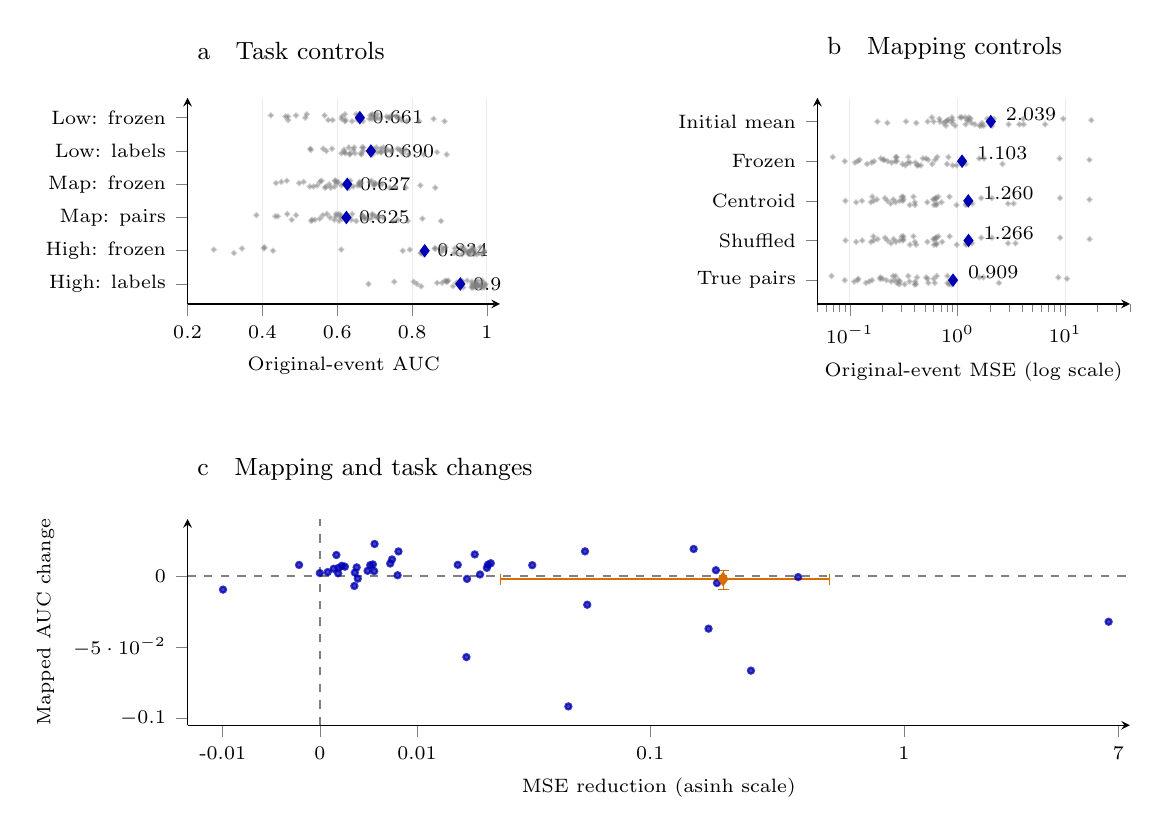
\begin{tikzpicture}
\begin{axis}[axis lines=left,tick align=outside,tick label style={font=\scriptsize},label style={font=\scriptsize},title style={font=\small,align=left},grid style={gray!15},every axis plot/.append style={line width=.8pt},enlarge x limits=false,at={(0cm,0cm)},anchor=north west,width=5.55cm,height=4.2cm,title={a\quad Task controls},title style={font=\small,align=left,at={(0,1.06)},anchor=south west},xlabel={Original-event AUC},xmin=.2,xmax=1.035,ymin=-.6,ymax=5.6,ytick={5,4,3,2,1,0},yticklabels={Low: frozen,Low: labels,Map: frozen,Map: pairs,High: frozen,High: labels},xmajorgrids=true]
\addplot[gray,only marks,mark=*,mark size=.65pt,opacity=.4] coordinates {(0.668723765432,4.895) (0.622220679012,4.93) (0.71500154321,4.965) (0.737311728395,5) (0.612604938272,5.035) (0.688425925926,5.07) (0.650436728395,5.105) (0.639442901235,4.895) (0.575901234568,4.93) (0.701672839506,4.965) (0.664,5) (0.75749382716,5.035) (0.694487654321,5.07) (0.659026234568,5.105) (0.818913580247,4.895) (0.771817901235,4.93) (0.68562345679,4.965) (0.740226851852,5) (0.760220679012,5.035) (0.746029320988,5.07) (0.620472222222,5.105) (0.620699074074,4.895) (0.587854938272,4.93) (0.857538580247,4.965) (0.70649845679,5) (0.468351851852,5.035) (0.489858024691,5.07) (0.518557098765,5.105) (0.88687345679,4.895) (0.654154320988,4.93) (0.693064814815,4.965) (0.764091049383,5) (0.731941358025,5.035) (0.566094135802,5.07) (0.707086419753,5.105) (0.785600308642,4.895) (0.468845679012,4.93) (0.611802469136,4.965) (0.514762345679,5) (0.461695987654,5.035) (0.422709876543,5.07) (0.693398148148,5.105)};
\addplot[gray,only marks,mark=*,mark size=.65pt,opacity=.4] coordinates {(0.694353395062,3.895) (0.647433641975,3.93) (0.715907407407,3.965) (0.744739197531,4) (0.618132716049,4.035) (0.696375,4.07) (0.669717592593,4.105) (0.664580246914,3.895) (0.622172839506,3.93) (0.718591049383,3.965) (0.669820987654,4) (0.783287037037,4.035) (0.715901234568,4.07) (0.66662808642,4.105) (0.831344135802,3.895) (0.775344135802,3.93) (0.696154320988,3.965) (0.744344135802,4) (0.767075617284,4.035) (0.76112345679,4.07) (0.645453703704,4.105) (0.633430555556,3.895) (0.611067901235,3.93) (0.866677469136,3.965) (0.729413580247,4) (0.52962191358,4.035) (0.527808641975,4.07) (0.630804012346,4.105) (0.892481481481,3.895) (0.663427469136,3.93) (0.707385802469,3.965) (0.77074845679,4) (0.734856481481,4.035) (0.585970679012,4.07) (0.723739197531,4.105) (0.790356481481,3.895) (0.634603395062,3.93) (0.619316358025,3.965) (0.570950617284,4) (0.642527777778,4.035) (0.562507716049,4.07) (0.704447530864,4.105)};
\addplot[gray,only marks,mark=*,mark size=.65pt,opacity=.4] coordinates {(0.631925925926,2.895) (0.593,2.93) (0.697101851852,2.965) (0.701970679012,3) (0.598483024691,3.035) (0.602617283951,3.07) (0.558012345679,3.105) (0.582691358025,2.895) (0.526569444444,2.93) (0.661212962963,2.965) (0.618814814815,3) (0.658601851852,3.035) (0.66024845679,3.07) (0.634782407407,3.105) (0.783114197531,2.895) (0.754572530864,2.93) (0.546591049383,2.965) (0.719828703704,3) (0.701942901235,3.035) (0.686938271605,3.07) (0.596091049383,3.105) (0.567399691358,2.895) (0.536649691358,2.93) (0.822035493827,2.965) (0.661114197531,3) (0.436341049383,3.035) (0.510228395062,3.07) (0.465429012346,3.105) (0.862097222222,2.895) (0.642896604938,2.93) (0.654820987654,2.965) (0.698549382716,3) (0.664271604938,3.035) (0.553581790123,3.07) (0.691708333333,3.105) (0.740200617284,2.895) (0.570233024691,2.93) (0.611049382716,2.965) (0.578969135802,3) (0.498337962963,3.035) (0.450584876543,3.07) (0.593336419753,3.105)};
\addplot[gray,only marks,mark=*,mark size=.65pt,opacity=.4] coordinates {(0.65087654321,1.895) (0.592195987654,1.93) (0.690046296296,1.965) (0.710695987654,2) (0.596404320988,2.035) (0.609098765432,2.07) (0.572734567901,2.105) (0.605171296296,1.895) (0.532591049383,1.93) (0.678509259259,1.965) (0.609194444444,2) (0.626365740741,2.035) (0.668171296296,2.07) (0.639824074074,2.105) (0.788787037037,1.895) (0.762134259259,1.93) (0.553722222222,1.965) (0.722523148148,2) (0.702429012346,2.035) (0.69450617284,2.07) (0.603901234568,2.105) (0.530302469136,1.895) (0.540677469136,1.93) (0.827706790123,1.965) (0.672699074074,2) (0.434430555556,2.035) (0.489978395062,2.07) (0.466438271605,2.105) (0.877231481481,1.895) (0.637912037037,1.93) (0.672032407407,1.965) (0.706652777778,2) (0.66662037037,2.035) (0.561313271605,2.07) (0.693550925926,2.105) (0.749101851852,1.895) (0.478475308642,1.93) (0.61462345679,1.965) (0.580984567901,2) (0.44125308642,2.035) (0.383984567901,2.07) (0.596682098765,2.105)};
\addplot[gray,only marks,mark=*,mark size=.65pt,opacity=.4] coordinates {(0.972686728395,0.895) (0.822666666667,0.93) (0.95100617284,0.965) (0.955202160494,1) (0.79412191358,1.035) (0.860532407407,1.07) (0.962240740741,1.105) (0.95149845679,0.895) (0.82525617284,0.93) (0.955115740741,0.965) (0.774962962963,1) (0.884285493827,1.035) (0.91424382716,1.07) (0.931802469136,1.105) (0.988072530864,0.895) (0.978615740741,0.93) (0.947364197531,0.965) (0.962646604938,1) (0.960098765432,1.035) (0.939294753086,1.07) (0.889625,1.105) (0.830307098765,0.895) (0.911722222222,0.93) (0.950013888889,0.965) (0.940452160494,1) (0.61075,1.035) (0.404135802469,1.07) (0.40550462963,1.105) (0.96537962963,0.895) (0.919186728395,0.93) (0.991987654321,0.965) (0.993192901235,1) (0.967041666667,1.035) (0.862135802469,1.07) (0.98186882716,1.105) (0.934058641975,0.895) (0.324024691358,0.93) (0.878195987654,0.965) (0.428311728395,1) (0.270229938272,1.035) (0.345541666667,1.07) (0.87962808642,1.105)};
\addplot[gray,only marks,mark=*,mark size=.65pt,opacity=.4] coordinates {(0.986375,-0.105) (0.909421296296,-0.07) (0.975547839506,-0.035) (0.967365740741,0) (0.866949074074,0.035) (0.891797839506,0.07) (0.974441358025,0.105) (0.962933641975,-0.105) (0.960814814815,-0.07) (0.981439814815,-0.035) (0.812969135802,0) (0.918674382716,0.035) (0.934313271605,0.07) (0.947145061728,0.105) (0.992098765432,-0.105) (0.983898148148,-0.07) (0.974097222222,-0.035) (0.970509259259,0) (0.988427469136,0.035) (0.95988117284,0.07) (0.930733024691,0.105) (0.937024691358,-0.105) (0.974484567901,-0.07) (0.969520061728,-0.035) (0.959898148148,0) (0.92187345679,0.035) (0.752304012346,0.07) (0.888353395062,0.105) (0.969956790123,-0.105) (0.927950617284,-0.07) (0.995680555556,-0.035) (0.996169753086,0) (0.972544753086,0.035) (0.893851851852,0.07) (0.98700462963,0.105) (0.958955246914,-0.105) (0.824351851852,-0.07) (0.925587962963,-0.035) (0.683544753086,0) (0.880490740741,0.035) (0.804558641975,0.07) (0.896594135802,0.105)};
\addplot[blue!70!black,only marks,mark=diamond*,mark size=1.8pt] coordinates {(0.660512676367,5) (0.690014844209,4) (0.626784428277,3) (0.624584141681,2) (0.833690696649,1) (0.928822236919,0)};
\node[anchor=west,font=\scriptsize] at (axis cs:0.668512676367,5) {0.661};
\node[anchor=west,font=\scriptsize] at (axis cs:0.698014844209,4) {0.690};
\node[anchor=west,font=\scriptsize] at (axis cs:0.634784428277,3) {0.627};
\node[anchor=west,font=\scriptsize] at (axis cs:0.632584141681,2) {0.625};
\node[anchor=west,font=\scriptsize] at (axis cs:0.841690696649,1) {0.834};
\node[anchor=west,font=\scriptsize] at (axis cs:0.936822236919,0) {0.929};
\end{axis}
\begin{axis}[axis lines=left,tick align=outside,tick label style={font=\scriptsize},label style={font=\scriptsize},title style={font=\small,align=left},grid style={gray!15},every axis plot/.append style={line width=.8pt},enlarge x limits=false,at={(8.0cm,0cm)},anchor=north west,width=5.55cm,height=4.2cm,title={b\quad Mapping controls},title style={font=\small,align=left,at={(0,1.06)},anchor=south west},xlabel={Original-event MSE (log scale)},xmode=log,xmin=.05,xmax=40,ymin=-.6,ymax=4.6,ytick={4,3,2,1,0},yticklabels={Initial mean,Frozen,Centroid,Shuffled,True pairs},xmajorgrids=true]
\addplot[gray,only marks,mark=*,mark size=.65pt,opacity=.4] coordinates {(2.10091914804,3.895) (6.51929444518,3.93) (0.745201017029,3.965) (0.528822266796,4) (1.23303364937,4.035) (0.679581941632,4.07) (0.887644253194,4.105) (0.950673908244,3.895) (1.19197028455,3.93) (1.68951058814,3.965) (0.686188252461,4) (17.5142767585,4.035) (4.06904738561,4.07) (1.17657260906,4.105) (1.75373429754,3.895) (1.45261144047,3.93) (0.223072795084,3.965) (0.600956984547,4) (1.26407851199,4.035) (2.17843583253,4.07) (1.27712689836,4.105) (0.780701234807,3.895) (4.11858495445,3.93) (1.34544169293,3.965) (0.332120142704,4) (0.899061251085,4.035) (1.32047720468,4.07) (0.577172150824,4.105) (1.66044748674,3.895) (2.98887999261,3.93) (0.413388183306,3.965) (0.7770370869,4) (0.809005195002,4.035) (1.88900539403,4.07) (1.05763571022,4.105) (1.60297346815,3.895) (3.75602113542,3.93) (0.888766343535,3.965) (0.180300149917,4) (0.819963818772,4.035) (9.60153455434,4.07) (1.09217124531,4.105)};
\addplot[gray,only marks,mark=*,mark size=.65pt,opacity=.4] coordinates {(0.981926788066,2.895) (1.19065188887,2.93) (0.244332589372,2.965) (0.225183050717,3) (0.208781752965,3.035) (0.19410678065,3.07) (0.267778714463,3.105) (0.328587487331,2.895) (0.144391399455,2.93) (0.346338947967,2.965) (0.273632682486,3) (16.8301418934,3.035) (1.76530518776,3.07) (0.349563309775,3.105) (0.421522515305,2.895) (0.307871273021,2.93) (0.111598912818,2.965) (0.118526318893,3) (0.534493831858,3.035) (1.59079053321,3.07) (0.823991359356,3.105) (0.457454914976,2.895) (2.61360560133,2.93) (0.406173910811,2.965) (0.167841514019,3) (0.204845732358,3.035) (0.476930257943,3.07) (0.271927621874,3.105) (0.430662955159,2.895) (0.798438189036,2.93) (0.158993428902,2.965) (0.264452175718,3) (0.123033847381,3.035) (0.509785398507,3.07) (0.0693453813614,3.105) (0.900734798013,2.895) (0.583033443417,2.93) (0.362853646838,2.965) (0.0896888153653,3) (0.619321160157,3.035) (8.89409780329,3.07) (0.64806881461,3.105)};
\addplot[gray,only marks,mark=*,mark size=.65pt,opacity=.4] coordinates {(1.19829239247,1.895) (3.31718177865,1.93) (0.265406326865,1.965) (0.223477241876,2) (0.315620371747,2.035) (0.211663861977,2.07) (0.313428449501,2.105) (0.360254085469,1.895) (0.239745673777,1.93) (0.709253508231,1.965) (0.309056648198,2) (16.8182082043,2.035) (2.08573107591,2.07) (0.390006295065,2.105) (0.604534590414,1.895) (0.642772962653,1.93) (0.11436399674,1.965) (0.129620099273,2) (0.59361454063,2.035) (1.65996094457,2.07) (0.842306881379,2.105) (0.403791947083,1.895) (2.947521708,1.93) (0.523321514471,1.965) (0.166671265506,2) (0.25320398208,2.035) (0.625745662049,2.07) (0.303273444125,2.105) (0.633636402247,1.895) (1.37157683218,1.93) (0.156770658076,1.965) (0.289709998308,2) (0.178920371881,2.035) (0.632898393438,2.07) (0.161789140561,2.105) (0.980563187545,1.895) (1.21222069198,1.93) (0.401570733669,1.965) (0.0909237644527,2) (0.612902427116,2.035) (8.9607331368,2.07) (0.663432887944,2.105)};
\addplot[gray,only marks,mark=*,mark size=.65pt,opacity=.4] coordinates {(1.19974142457,0.895) (3.46072318183,0.93) (0.267376934973,0.965) (0.224198572834,1) (0.314233873238,1.035) (0.212114136094,1.07) (0.314309019997,1.105) (0.361995389561,0.895) (0.241106388341,0.93) (0.720858603334,0.965) (0.311888619079,1) (16.8580408386,1.035) (2.08939257574,1.07) (0.390276866415,1.105) (0.604558879909,0.895) (0.637087614403,0.93) (0.114490044654,0.965) (0.130147690891,1) (0.595356439812,1.035) (1.6627858905,1.07) (0.844155466122,1.105) (0.413394456071,0.895) (2.95201683825,0.93) (0.525190418193,0.965) (0.166913181189,1) (0.255063734642,1.035) (0.628102707305,1.07) (0.30428027334,1.105) (0.637194009793,0.895) (1.36437588766,0.93) (0.157118510918,0.965) (0.290920671217,1) (0.181173029515,1.035) (0.633644899713,1.07) (0.165373072877,1.105) (0.983454301554,0.895) (1.20966878902,0.93) (0.401918299441,0.965) (0.0909677211198,1) (0.613356704955,1.035) (8.98519423244,1.07) (0.665404724332,1.105)};
\addplot[gray,only marks,mark=*,mark size=.65pt,opacity=.4] coordinates {(0.833488404516,-0.105) (0.807306318333,-0.07) (0.241144324295,-0.035) (0.218351745422,0) (0.191088433322,0.035) (0.191808502994,0.07) (0.266269631645,0.105) (0.323412878299,-0.105) (0.140983393309,-0.07) (0.291341033584,-0.035) (0.283585103688,0) (10.4180369769,0.035) (1.74340723939,0.07) (0.348300314661,0.105) (0.399851780614,-0.105) (0.274237445965,-0.07) (0.109585651689,-0.035) (0.117809291662,0) (0.52683378275,0.035) (1.5860572135,0.07) (0.807944496559,0.105) (0.28754287512,-0.105) (2.43188371942,-0.07) (0.404468031833,-0.035) (0.160811210812,0) (0.201329581421,0.035) (0.420783316436,0.07) (0.251704948517,0.105) (0.411498646757,-0.105) (0.614900067688,-0.07) (0.151235526216,-0.035) (0.259447512602,0) (0.119799902244,0.035) (0.511679488679,0.07) (0.0676779279193,0.105) (0.878209246151,-0.105) (0.535875218757,-0.07) (0.358383893793,-0.035) (0.0896863136232,0) (0.601733532877,0.035) (8.6443027699,0.07) (0.642935289467,0.105)};
\addplot[blue!70!black,only marks,mark=diamond*,mark size=1.8pt] coordinates {(2.03889146819,4) (1.10263825307,3) (1.25989709712,2) (1.26618011701,1) (0.908731737699,0)};
\node[anchor=west,font=\scriptsize] at (axis cs:2.28355844438,4.19) {2.039};
\node[anchor=west,font=\scriptsize] at (axis cs:1.23495484343,3.19) {1.103};
\node[anchor=west,font=\scriptsize] at (axis cs:1.41108474878,2.19) {1.260};
\node[anchor=west,font=\scriptsize] at (axis cs:1.41812173105,1.19) {1.266};
\node[anchor=west,font=\scriptsize] at (axis cs:1.01777954622,0.19) {0.909};
\end{axis}
\begin{axis}[axis lines=left,tick align=outside,tick label style={font=\scriptsize},label style={font=\scriptsize},title style={font=\small,align=left},grid style={gray!15},every axis plot/.append style={line width=.8pt},enlarge x limits=false,at={(0cm,-5.35cm)},anchor=north west,width=13.55cm,height=4.2cm,title={c\quad Mapping and task changes},title style={font=\small,align=left,at={(0,1.06)},anchor=south west},xlabel={MSE reduction (asinh scale)},ylabel={Mapped AUC change},xmin=-1.2,xmax=7.35,ymin=-.105,ymax=.04,xtick={-0.88137358702,0,0.88137358702,2.9982229503,5.29834236561,7.24422802581},xticklabels={-0.01,0,0.01,0.1,1,7}]
\addplot[gray,dashed] coordinates {(-1.2,0) (7.35,0)};
\addplot[gray,dashed] coordinates {(0,-0.105) (0,0.04)};
\addplot[blue!70!black,only marks,mark=*,mark size=1.1pt,opacity=.75] coordinates {(3.39186472048,0.018950617284) (4.33966902095,-0.000804012345679) (0.313658127458,-0.00705555555556) (0.638791803381,0.00872530864198) (1.33544935549,-0.0020787037037) (0.227851116901,0.00648148148148) (0.150341293065,0.0147222222222) (0.4967745452,0.0224799382716) (0.334526259212,0.00602160493827) (2.40602181596,0.0172962962963) (-0.87800525304,-0.00962037037037) (7.15650557172,-0.0322361111111) (1.52542943278,0.00792283950617) (0.125966119885,0.00504166666667) (1.51595026688,0.00567283950617) (1.92749557644,0.00756172839506) (0.199990304874,0.00713117283951) (0.0716414241913,0.00269444444444) (0.705901957423,0.000486111111111) (0.457232935602,0.00756790123457) (1.25146443854,0.00781018518519) (3.52670780324,-0.0370972222222) (3.59379567797,0.00402777777778) (0.169771190275,0.0056712962963) (0.655147334381,0.0115848765432) (0.344745590475,-0.00191049382716) (2.42637185896,-0.02025) (1.453549611,0.00100925925926) (1.4056251593,0.0151342592593) (3.60372579719,-0.00498456790123) (0.713651822041,0.0172114197531) (0.48162886795,0.00810339506173) (0.318007399947,0.0023487654321) (-0.188294387178,0.00773148148148) (0.165982156827,0.00184259259259) (1.55119522448,0.0089012345679) (2.25512708176,-0.0917577160494) (0.433289824648,0.00357407407407) (0.000250174206506,0.00201543209877) (1.33023710938,-0.0570848765432) (3.91160321886,-0.066600308642) (0.493122672202,0.00334567901235)};
\addplot+[orange!85!black,only marks,mark=diamond*,mark size=2pt,error bars/.cd,x dir=both,x explicit,y dir=both,y explicit] coordinates {(3.65860248705,-0.00220028659612) += (0.968945901145,0.00622148736038) -= (2.01973128316,0.00747527006173)};
\end{axis}
\end{tikzpicture}
\caption{Original-event controls and participant-level outcomes in Lee's 42-person confirmation group. (a,b) Gray points show individual outcomes, and blue diamonds show equal-participant means. The logarithmic MSE axis includes all extreme values. High-view classifiers use 62 observed channels with either frozen or label-updated readouts. Mapped classifiers combine observed Cz/Pz features with predictions for the omitted channels, using the original fixed high-view readout. (c) Each point shows one participant's MSE reduction and mapped AUC change relative to frozen mapping. The orange diamond and whiskers show aggregate means and the original marginal 95\% intervals, which do not form a joint confidence region. Positions use $\operatorname{asinh}(\mathrm{MSE\ reduction}/0.01)$, with ticks labeled in original units. Figure~\ref{fig:eeg-lee-history} reports the separate common-history event set and its complete controls.}
\label{fig:eeg-lee-endpoints}
\end{figure}
